\documentclass[10pt]{article}
\usepackage{icmlko}

\icmlmeta{IP 파운데이션 월드모델}{209}{달력이 판의 4분의 1인데 모형은 달력을 안 본다}{축의 정의에 시간이 들었는지 봤으니 라벨도 봤다. 여섯 도메인의 라벨이 시간을 담고 있고 ``언제 나왔나''만으로 판의 4분의 1이 나온다 --- 그런데 모형은 거기 안 기댄다}

\begin{document}

\twocolumn[
\icmlheader

\begin{abstract}
노트 207 · 208이 \emph{축}의 정의에 측정 시각이 들었는지 훑었다. 라벨은
안 봤다. \textbf{봤더니 축보다 심하다.} 열 도메인 중 \textbf{여섯}에서
라벨이 시작 연도와 $-$0.15 보다 세게 붙는다 --- 게임 \textbf{$-$0.648}
(스팀 리뷰 누적) · 도서 $-$0.579 · 웹툰 $-$0.352 · 애니 $-$0.323 · 펀딩
$-$0.272 · 만화 $-$0.158. \textbf{옛것이 높다} --- 누적 라벨은 오래 모을수록
크기 때문이다. 유보 안(2025$\sim$26, 두 해)에서도 게임 $-$0.494 · 도서
$-$0.562 로 강하다. 유일한 양수가 아이돌($+$0.367)인데 그 라벨은 \emph{초동
판매} --- 고정 창이라 시간에 안 눕는다. \textbf{그래서 극단 기준선을 쟀다}:
``\textbf{$-$시작일}'' 하나만 예측으로 쓰면 판 $\rho$ 가 \textbf{$+$0.2513}
이다(우연 $+$0.0126). 도서 $+$0.562 · 게임 $+$0.494 · 아이돌 $+$0.358 ·
웹툰 $+$0.350 --- \textbf{두 도메인은 유보 순위가 사실상 달력이다.}
\textbf{여기서 이 노트가 갈린다.} 시간을 빼고 다시 쟀다 --- 유보를 반년
코호트로 잘라 코호트 \emph{안}에서만 $\rho$ 를 내고 표본 수로 가중한다.
\textbf{시작일 기준선은 $+$0.2513 에서 $+$0.1396 으로 반 토막인데 모형은
안 움직인다} --- F6 능형 $+$0.4092 $\to$ \textbf{$+$0.4095}, F21 $+$0.4219
$\to$ $+$0.4227, F18 배깅 $+$0.4614 $\to$ $+$0.4397. \textbf{선형은 한 자리도
안 움직이고 트리만 $-$0.022 잃는다.} 그러니 결론이 둘이다:
\textbf{① 판 $\rho$ 의 4분의 1은 ``언제 나왔나''로 설명된다}(그리고 그것은
라벨이 안 여문 것이지 세계가 아니다). \textbf{② 그런데 모형이 이기는 것은
그것 때문이 아니다} --- 달력을 빼도 모형의 우위가 그대로다.
\end{abstract}
]

\begin{figure*}[t]
\centering
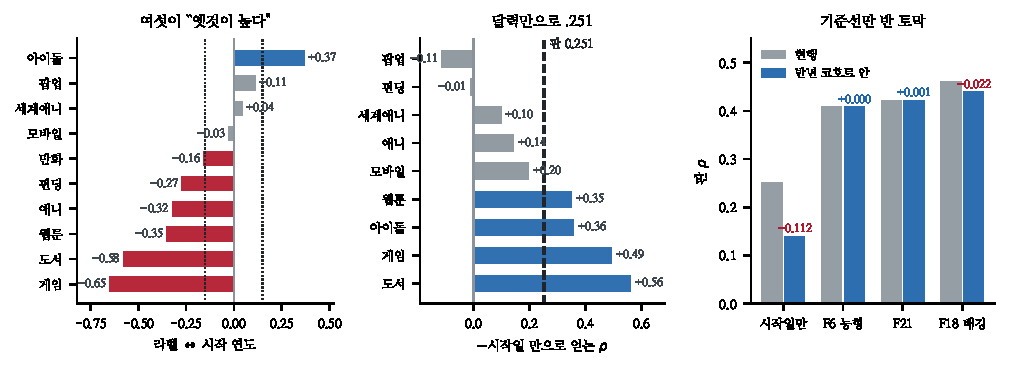
\includegraphics[width=\textwidth]{figs/clock.pdf}
\caption{왼쪽 --- 여섯이 ``옛것이 높다''. 가운데 --- 달력만으로 .251.
오른쪽 --- 기준선만 반 토막.}
\end{figure*}

\section{라벨이 시간을 담는다}

\begin{table}[t]
\centering\tsize
\caption{라벨 $\leftrightarrow$ 시작 연도.}
\begin{tabular}{lrrl}
\toprule
& 전체 & 유보 안 & 라벨 \\
\midrule
\textbf{게임} & \textbf{$-$.648} & $-$.494 & 스팀 리뷰 누적 \\
\textbf{도서} & \textbf{$-$.579} & $-$.562 & 알라딘 판매지수 \\
웹툰 & $-$.352 & $-$.350 & 즐겨찾기 누적 \\
애니 & $-$.323 & $-$.144 & 라프텔 지표 \\
펀딩 & $-$.272 & $+$.012 & 후원자(마감) \\
만화 & $-$.158 & --- & 인기도 누적 \\
\midrule
\textbf{아이돌} & \textbf{$+$.367} & $-$.358 & \textbf{초동(고정 창)} \\
\bottomrule
\end{tabular}
\end{table}

\claimx{\textbf{여섯이 ``옛것이 높다''}이고 그 여섯은 전부 누적 지표다 ---
리뷰 수 · 판매지수 · 즐겨찾기 · 인기도. 오래 나와 있을수록 더
모았다.}{\textbf{유일한 양수가 아이돌이고 그 라벨만 고정 창이다}(초동 1주).
\textbf{라벨의 창이 고정이면 시간에 안 눕는다} --- 우연이라기엔 너무
깨끗한 대조다.}

\claimx{\textbf{유보 두 해 안에서도 강하다}(게임 $-$0.494 · 도서 $-$0.562).
2025년 초에 나온 것과 2026년 중반에 나온 것 사이에도 누적 시간이 배
넘게 차이 난다.}{그러니 ``유보를 시간으로 잘랐으니 안전하다''가 아니다 ---
\textbf{자른 안쪽에도 시계가 돈다.}}

\section{달력만으로 4분의 1}

\begin{table}[t]
\centering\tsize
\caption{예측 $=$ $-$시작일. 그것뿐.}
\begin{tabular}{lrr}
\toprule
& 유보 n & $\rho$ \\
\midrule
\textbf{도서} & 163 & \textbf{$+$.562} \\
\textbf{게임} & 223 & \textbf{$+$.494} \\
아이돌 & 25 & $+$.358 \\
웹툰 & 711 & $+$.350 \\
모바일 & 441 & $+$.198 \\
애니 & 606 & $+$.144 \\
세계애니 & 300 & $+$.099 \\
팝업 & 59 & $-$.113 \\
\midrule
\textbf{판} & 2{,}608 & \textbf{$+$.2513} \\
(우연) & & $+$.0126 \\
\bottomrule
\end{tabular}
\end{table}

\claimx{\textbf{도서와 게임은 유보 순위가 사실상 달력이다}($+$0.562 ·
$+$0.494). 축을 하나도 안 보고 날짜만 봐도 그만큼 맞힌다.}{\textbf{그리고
그것은 세계에 관한 사실이 아니다} --- 2026년 게임이 2025년 게임보다 못한
것이 아니라 리뷰를 덜 모은 것이다. \textbf{판이 재는 것에 측정 시계가
섞여 있다.}}

\section{그런데 모형은 달력을 안 본다}

\begin{table}[t]
\centering\tsize
\caption{유보를 반년 코호트로 잘라 코호트 안에서만.}
\begin{tabular}{lrrr}
\toprule
& 현행 & 코호트 안 & 차 \\
\midrule
\textbf{시작일만} & \textbf{.2513} & \textbf{.1396} & \textbf{$-$.112} \\
\midrule
F6 능형 & .4092 & \textbf{.4095} & $+$.000 \\
F21 & .4219 & \textbf{.4227} & $+$.001 \\
F18 배깅 & .4614 & .4397 & $-$.022 \\
우연 & .0126 & .0082 & $-$.004 \\
\bottomrule
\end{tabular}
\end{table}

\claimx{\textbf{기준선은 반 토막인데 선형 모형은 한 자리도 안 움직인다.}
달력 정보를 45\% 없앴는데 F6 는 $+$0.0003 오른다.}{\textbf{모형의 우위가
달력에서 오는 것이 아니라는 증거다.} 걱정한 것이 실재하지만 걱정한 만큼은
아니다.}

\claimx{\textbf{트리만 $-$0.022 잃는다.} 노트 186이 ``트리는 도메인으로
쪼갠 뒤 열끼리 곱한다''를 쟀는데, 달력 축 여섯이 그 재료 중 하나다(노트
186의 트리 우위 $+$0.140).}{그래도 코호트 안에서 F18 이 $+$0.4397 로
여전히 제일 높다 --- \textbf{순위는 안 바뀐다.}}

\claimx{\textbf{그러니 판정치를 안 바꾼다.} 코호트 안 $\rho$ 가 더 옳아
보이지만 순위가 같고, 판정치를 점수 보고 바꾸는 것이 노트 82 · 90 이 금한
것이다.}{\textbf{대신 나란히 적을 값은 있다} --- 노트 184가 가중 셋을
견줬을 때와 같은 이유로, 이건 판정치의 성질을 아는 데 쓰인다.}

\begin{table}[t]
\centering\tsize
\caption{남은 것.}
\begin{tabular}{ll}
\toprule
\textbf{게임·도서} & 유보 $\rho$ 의 절반이 달력 --- 라벨을 고칠 수 있나 \\
아이돌 & 고정 창 라벨이라 안 눕는다 --- 다른 도메인도 \\
트리 & $-$0.022 --- 달력 축을 얼마나 쓰나 \\
\bottomrule
\end{tabular}
\end{table}

첫 줄이 자료 쪽으로 열려 있고 값이 크다. 게임 라벨은 스팀 리뷰 \emph{누적}
수인데, 스팀 API 는 리뷰를 날짜별로 준다 --- \textbf{출시 후 90일 창으로
자르면 아이돌의 초동처럼 시간에 안 눕는 라벨이 된다.} 도서의 알라딘
판매지수도 기간 지정이 가능하다. \textbf{라벨을 고정 창으로 바꾸면 판의
4분의 1을 차지하던 달력이 사라지고, 남는 것이 진짜 신호다.} 다만 그것은
BQ/GCP 가 아니라 바깥 API 를 다시 긁는 일이라 이 사이클에서는 못 한다 ---
\textbf{다음 수집 때 반드시 할 것으로 적어 둔다.}

\end{document}
